\section{Introduction}
\label{sec:intro}

Agent benchmarks and training loops rarely consume raw model generations. They consume an action
produced by a chain: emission $\rightarrow$ serialization $\rightarrow$ parse $\rightarrow$
execution $\rightarrow$ observation $\rightarrow$ score or reward. A failure at several of these
boundaries has the same observable as a model declining to act: HTTP 200 and an empty
\texttt{tool\_calls} array. We call the resulting measurement failure \emph{interface-induced
trajectory censoring}. The term covers two distinct effects: \emph{masking}, where a tool-intended
emission never enters the structured action channel, and \emph{suppression}, where an interface
constraint prevents an invalid action from entering that channel. Their common methodological
problem is not a shared mechanism but a shared terminal observation that is easily attributed to
the model. Figure~\ref{fig:funnel} shows the layers measured in our experiments.

\begin{figure}[t]
\centering
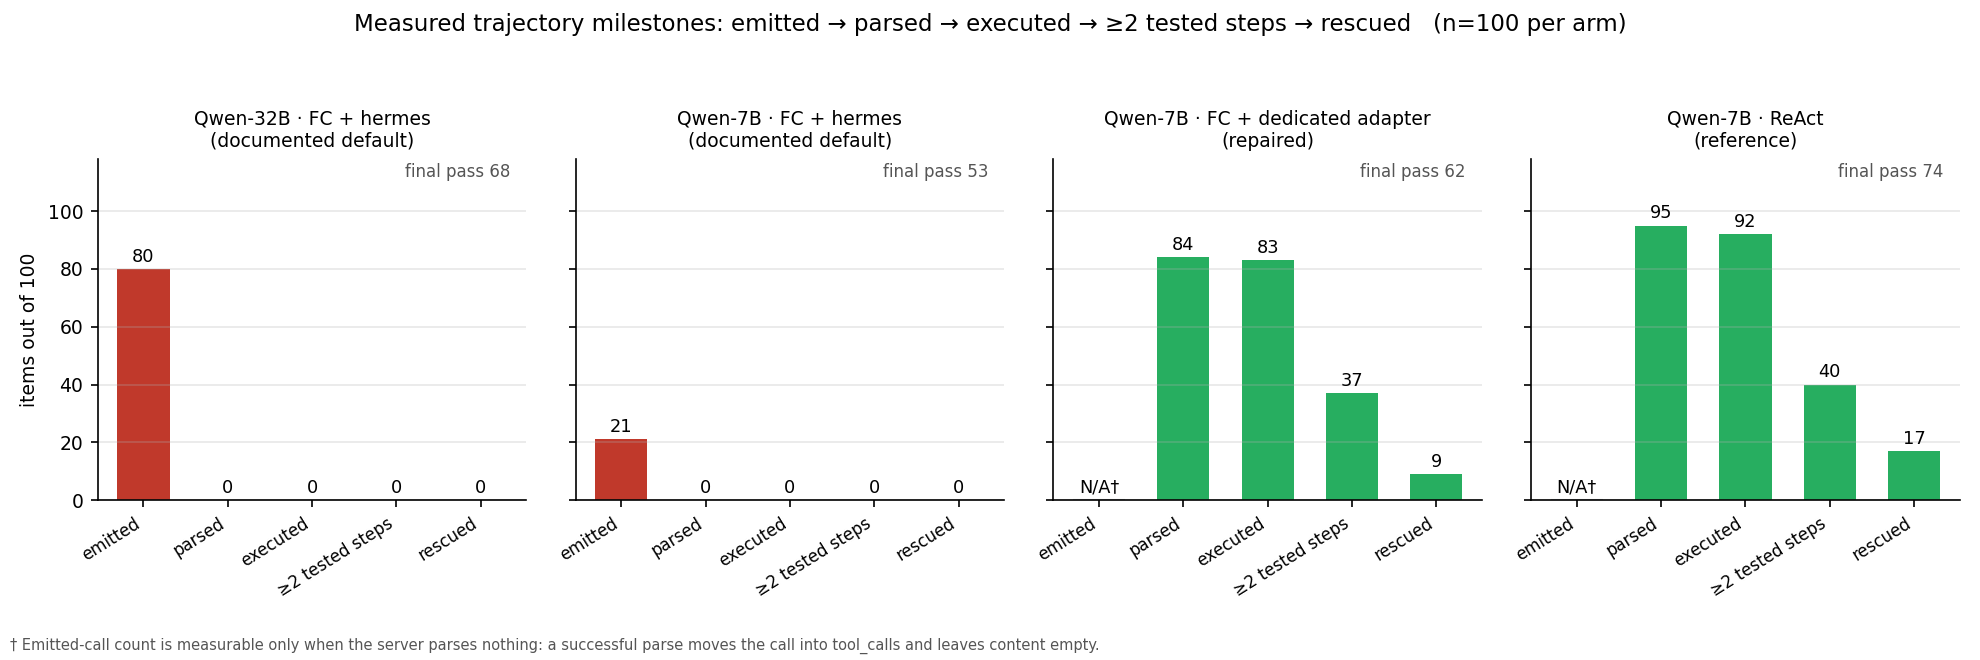
\includegraphics[width=0.92\linewidth]{fig0_funnel.png}
\caption{A tool-use measurement funnel. Calls present in raw generations can disappear before
parsing, execution, observation, or scoring. N/A denotes cells that cannot be read from content
once the server has moved a successful call into \texttt{tool\_calls}.}
\label{fig:funnel}
\end{figure}

Historical 1.5B runs motivated the investigation, but their ambiguous zero-execution result
does not identify parser masking (Appendix~\ref{app:extra}). We instead organize the evidence
around benchmark measurement, component interventions and the formal 7B control of training
experience, with explicit limits on what each observation identifies.

The individual Qwen incompatibility was reported previously in vLLM issue \#32926
\citep{vllm_issue_32926}. Our contribution is to quantify it as an evaluation-validity failure,
decompose its causes, and follow it into interactive evaluation and RL:
\begin{itemize}
\setlength{\itemsep}{1pt}
\item On BFCL v4, a template--parser $2\times2$ shows zero recovery from either one-component
replacement at the documented baseline and 196/200 parses when both are replaced; on
$\tau$-bench, the same joint repair restores 636 executions over 115 tasks.
\item A five-checkpoint ladder measures a growing absolute undercount under one mismatched
interface, while a preregistered matched-interface ladder keeps the silent fraction at 0--2.
\item A paired Llama intervention shows the opposite interface effect: relative to the
official-template baseline, \texttt{strict: true} suppresses 22 wrong-tool calls and raises final
pass from 44 to 61.
\item A preregistered 7B RL control changes only verl's parser registry. Repair restores 16,844
executed and observed calls, but no held-out improvement is detected, separating access to
experience from learning from it.
\end{itemize}

The resulting claim is narrower than ``the stack matters.'' A serving interface is part of both
the benchmark's measurement function and an agent's effective action space. Consequently,
tool-use results require layer-wise observability and a conformance check before model or protocol
attribution.

\section{Related Work}
\label{sec:related}

Evaluation outcomes vary with prompt format, benchmark choice, and other nuisance factors
\citep{sclar2024formatspread,mizrahi2024stateofwhatart,dehghani2021benchmarklottery}. Tool-use
audits similarly expose evaluator defects and ambiguous failure attribution
\citep{bhat2026benchmarkingbenchmarks,raj2026modelorharness,soni2026toolfailbench,albayaydh2026beyondleaderboard}.
Those studies generally vary inputs or inspect traces above the serving boundary. We study a
component inside the measurement apparatus: an independently configured serialization--parser
contract that can erase an action without an error. The closest analogue is a security-log study
where reparsing identical bytes changes measured accuracy from 0\% to 76\%
\citep{garware2026brokenruler}. We extend that structure to standard agent benchmarks, downstream
execution, and RL experience. Harness-Bench argues for reporting model--harness configurations
from cross-harness workflow measurements \citep{yao2026harnessbench}; we isolate one contract with
component-level interventions and follow it into training. Agent-Reactive Bugs finds silent
model--harness boundary failures in issue reports \citep{chen2026agentreactive}; our evidence is a
controlled intervention rather than a bug-report taxonomy. BFCL~\citep{bfcl2025}, $\tau$-bench~\citep{yao2025taubench}, and
other tool benchmarks~\citep{qin2024toolllm,li2023apibank} supply the evaluation context; verl
~\citep{sheng2025hybridflow}, GRPO~\citep{shao2024deepseekmath}, and LoRA~\citep{hu2022lora}
supply the training stack. Constrained generation can hurt reasoning
\citep{tam2024speakfreely}; our Llama control is a complementary case in which a constraint removes
role confusion and improves execution.

\section{Framework and Testable Signatures}
\label{sec:framework}

Let $Y$ be the assistant bytes produced from fixed weights, prompt, and decoding; $C(Y)$ an
independent indicator that those bytes contain a tool-intended action; $P(Y)$ the structured action
returned by the configured parser; and $E(P(Y))$ the execution and observation produced by the
environment. A benchmark normally records a function of $P(Y)$ or $E(P(Y))$, not $Y$. We call an
item \emph{masked} when $C(Y)=1$ but $P(Y)=\varnothing$. This definition avoids a metaphysical
``true capability'': the directly observed fact is that a behavior exists in the raw generation
and is absent from the structured trace. It also does not imply a parser bug. The parser may
correctly reject bytes outside its grammar; the invalid measurement arises when checkpoint,
template, and parser are treated as a compatible bundle without testing their contract.

The framework gives three diagnostic signatures. First, a parser-only intervention cannot change
bytes already generated, but can change execution, observations, later turns, and rescues. Our
evaluation-time Qwen repair changes parser, template, and few-shot together, so its identical
aggregate turn-1 count (53 versus 53) is a consistency check, not layer identification. We instead
localize the failure with fixed-output replay and event tracing. Llama's \texttt{strict:true}
intervention acts earlier by constraining generation and therefore can change turn-1 output.

Second, a size trend in $C(Y)-\mathbb{1}[P(Y)\neq\varnothing]$ requires both changing emissions
and a fixed rejection boundary. Across a comparable scale span, our preregistered Qwen3 ladder
under a matched envelope does not show the same growth. This supporting cross-family observation
does not isolate family from envelope and is not a strict scale counterfactual. Third, in RL the parser
changes the sampled experience distribution before a policy-gradient estimator sees it. Restoring
actions and observations establishes access to tool-mediated experience, not a measured
gradient contribution or eventual learning. The formal 7B control tests the two claims separately: event counts identify
experience access, while held-out checkpoints test whether that access changes behavior.

\section{Measurement Setup}
\label{sec:setup}
\label{sec:control}
\label{sec:gating}

Our controlled probe uses 100 KodCode problems~\citep{kodcode2025}, decontaminated against
EvalPlus by normalized text/code n-gram containment, paired across arms, with one
\texttt{run\_tests(code)} tool. Function calling uses
\texttt{tool\_choice:auto}, temperature 0, and 2,048 output tokens. We separately run BFCL v4 at
pinned Gorilla commit \texttt{6ea5797} and all 115 $\tau$-bench \texttt{retail} tasks. The latter
uses a locally served Llama-3.1-8B user simulator rather than the original harness's
\texttt{gpt-4o}; its absolute score is therefore not leaderboard-comparable, and we claim only
paired arm differences.

Serving uses vLLM 0.27.1~\citep{kwon2023vllm}. Server-parsed calls are insufficient for the
question under study. One shared classifier marks a
generation \emph{tight} using a regex for a call-shaped payload naming \texttt{run\_tests},
a quoted \texttt{arguments.code} field and Python-like lexical markers. This heuristic rejects
some schema echoes and placeholders but does not validate JSON syntax or Python executability. Against a third-party-adjudicated gold standard its $\kappa$ is 0.871, and tight-stratum
precision is 36/40=0.900. Two annotators achieve $\kappa=0.967$ on the 62 items presented with
identical bytes. Stored evaluation outputs have a 4,000-character cap, which creates false
negatives, while 0.900 precision establishes false positives; the net bias is therefore not
identified. In the stratified validation sample, cap hits by scale are 0/6, 0/13, 0/15, 0/24,
and 10/40 from 1.5B through 32B, so truncation uncertainty is concentrated at the headline rung.
Formal RL rollouts are retained in full with hashes. Full validation appears in
Appendix~\ref{app:humanval}.

Before interpreting a zero we verify that \texttt{tool\_choice:required} produces a correctly
named, parseable call on the same live server. An arm enters pass-rate analysis only with 100
items, exit code 0, zero request errors, and matching provenance; this gate is enforced in code.
Appendix~\ref{app:errata} records an earlier invalid $p=0.648$ that this rule forced us to withdraw.

For paired binary outcomes we use exact two-sided McNemar tests and report both discordant counts;
for the formal RL endpoint we report a conservative finite-sample 95\% paired-risk interval
formed from exact binomial bounds on the two discordance probabilities. It reflects item-pair
uncertainty, not seed or inference-retest variation. Our explicit retrospective family has 27 tests
($0.05/27\approx0.00185$; Appendix~\ref{app:statistics}); this policy was not preregistered. We
distinguish a mechanism count (parse, execution, observation) from a task outcome throughout: a
large deterministic movement in the former does not license a performance claim when the paired
outcome test is null. BFCL scores come from its official scorer; $\tau$-bench outcomes come from
final environment state; code-task outcomes execute the generated program against held-out tests.
Training events exclude evaluation requests. Historical 1.5B curves exclude two verified
EvalPlus defects (\texttt{HumanEval/32} and \texttt{Mbpp/599}) and use $n=540$. The preregistered
7B control retains all 542 items and scores those two as failures in both arms; they affect
absolute rates but not paired discordances.

\section{Results}
\label{sec:results}

\subsection{External validity: BFCL and $\tau$-bench}
\label{sec:bfcl}
\label{sec:tau}

Holding model weights, cases, decoding, seeds, executor, and scorer fixed on BFCL v4, the
documented Hermes configuration yields official scores 0.00 on both \texttt{simple\_python} and
\texttt{multi\_turn\_base}; the dedicated Qwen2.5-Coder adapter yields 0.96 and 0.19. Because the
adapter changes both template and parser, we ran the full $2\times2$ (Table~\ref{tab:bfcl2x2}).
Changing either component alone from the documented baseline recovers none (0/200); changing both
recovers 196/200. Thus the two one-factor simple effects at that baseline are zero, while the joint
replacement shows strong complementarity. This statement concerns parse counts; official BFCL
scores were computed for the two end-to-end corner configurations, not all four cells. Each
component behaves according to its own contract, but the contracts disagree. The documented arm has zero HTTP errors and 166/200 strict
call emissions despite zero parses. On \texttt{multi\_turn\_base}, repair moves execution from
0 to 98/100 and success from 0 to 19/100. Complete scorer and funnel tables are in
Appendix~\ref{app:extra}.

\begin{table}[H]
\caption{BFCL first-request parses, template $\times$ parser ($n=200$).}
\label{tab:bfcl2x2}
\centering
\small
\begin{tabular}{lcc}
\toprule
 & documented template & dedicated template \\
\midrule
Hermes parser & 0 & 0 \\
Dedicated parser & 0 & \textbf{196} \\
\bottomrule
\end{tabular}
\end{table}

On paired $\tau$-bench tasks, the same adapter swap moves parsed and executed calls from
0 to 636 and tasks reaching any execution from 0/115 to 103/115. All 1,389 documented-arm
requests carry tools; 789 assistant turns contain call-shaped payloads that are not parsed.
Replaying vLLM's extractor classifies all 789 as missing the required envelope, with zero malformed
payloads and zero cases the parser should have accepted. Outcomes move from 7 to 10 solved, with
three discordant pairs in the repaired direction ($p=0.25$); we make no outcome claim. This result
extends the envelope-layer mechanism to a non-code, stateful environment, but not the scale or RL
claims, which remain code-only (Table~\ref{tab:external_main}).

\begin{table}[H]
\caption{External benchmarks under documented and repaired adapters. BFCL rows are official
scores; $\tau$-bench rows are paired counts over 115 tasks.}
\label{tab:external_main}
\centering
\small
\begin{tabular}{lrr}
\toprule
measurement & documented & repaired \\
\midrule
BFCL \texttt{simple\_python} score & 0.00 & \textbf{0.96} \\
BFCL \texttt{multi\_turn\_base} score & 0.00 & \textbf{0.19} \\
BFCL multi-turn executed/succeeded & 0/0 & \textbf{98/19} \\
\midrule
$\tau$-bench parsed/executed calls & 0/0 & \textbf{636/636} \\
$\tau$-bench tasks reaching a tool & 0 & \textbf{103} \\
$\tau$-bench tasks solved & 7 & 10 \\
\bottomrule
\end{tabular}
\end{table}

\subsection{Scale under mismatched and matched interfaces}
\label{sec:scale}

Under the documented Hermes interface, the Qwen2.5-Coder server reports zero calls at all five
sizes while tight-classified emissions rise monotonically from 0 to 80/100
(Table~\ref{tab:ladders}). A sensitivity estimate is approximately 72 if tight-stratum
precision transfers across sizes; this does not restore false negatives or estimate all true calls. A random 300-item
replication gives 0, 4, 30, 40, and 81 per 100: the 7B rung moves from 21 to 30, but direction and
monotonicity remain. This is a within-family observation under one mismatch, not a scaling law;
the server column is constant, so the slope comes entirely from increasingly frequent or regular
emissions. The 4,000-character cap creates false negatives, while classifier precision below one
creates false positives; the raw count's net bias is not identified.

The preregistered supporting ladder uses Qwen3 checkpoints up to 8B whose required envelope matches Hermes.
The prediction ``parsed $>0$ at every size'' was committed before inference. It holds, while the
silent fraction stays 1, 1, 2, and 0 through 8B; the separate mismatched ladder reaches 80 at
32B. This cross-family observation is
consistent with contract mismatch, rather than size alone, driving the undercount; it does not
isolate the envelope because family and envelope change together. Parsed counts are not monotone, and we disabled thinking because the
default exhausted the token budget before a call; both facts were recorded as protocol deviations.
An attempted Granite rescue produced no calls under either Hermes or its native parser and is
uninformative, not confirmatory.

\begin{table}[H]
\caption{Scale ladders. Tight counts concern unparsed outputs only (including Qwen3); they are not total emitted-call counts. ``Silent'' denotes these classifier-positive, unparsed outputs.}
\label{tab:ladders}
\label{tab:scale}
\centering
\small
\begin{tabular}{llrrr}
\toprule
family/interface & size & parsed & tight & silent \\
\midrule
Qwen2.5-Coder/Hermes & 1.5B & 0 & 0 & 0 \\
 & 3B & 0 & 4 & 4 \\
 & 7B & 0 & 21 & 21 \\
 & 14B & 0 & 36 & 36 \\
 & 32B & 0 & 80 & 80 \\
\midrule
Qwen3/matched & 0.6B & 86 & 1 & 1 \\
 & 1.7B & 44 & 1 & 1 \\
 & 4B & 70 & 2 & 2 \\
 & 8B & 97 & 0 & 0 \\
\bottomrule
\end{tabular}
\end{table}

A within-lineage Qwen2.5-Instruct control further localizes the effect: under the same template,
parser, items, and decoding, parsed rates are 1, 11, 63, 77, and 88 rather than Coder's flat zero.
After rerunning with a working executor, multi-turn rescues rise 0, 3, 6, 14, and 23 with that
parsed column. The contrast is consistent with checkpoint-specific post-training differences,
not parameter count or the shared family/template alone; it does not identify tool-format training
as the unique cause. Across 4,254 de-duplicated first turns from all archived arms, replay finds
zero cases that vLLM's configured parser should have accepted but did not: this is contract
mismatch, not a parser implementation bug (Table~\ref{tab:instruct_main}).

\begin{table}[H]
\caption{Within-lineage Qwen2.5-Instruct control under the same interface and items. Rescues are
final passes not passing on turn 1.}
\label{tab:instruct_main}
\centering
\small
\begin{tabular}{lrrrr}
\toprule
size & parsed & turn-1 & final & rescues \\
\midrule
1.5B & 1 & 13 & 13 & 0 \\
3B & 11 & 14 & 17 & 3 \\
7B & 63 & 34 & 40 & 6 \\
14B & 77 & 38 & 52 & 14 \\
32B & 88 & 42 & 65 & 23 \\
\bottomrule
\end{tabular}
\end{table}

\subsection{Llama: a constraint suppresses the wrong action}
\label{sec:llama}
\label{sec:taxonomy}
\label{sec:families}

Llama-3.1-8B calls the function requested by the programming problem rather than
\texttt{run\_tests} on 23/100 items. A richer schema leaves 22 wrong calls (discordances 6/5,
$p=1.0$), a thought scaffold worsens them to 59 ($p=2.84\times10^{-10}$), and the official
template leaves 22 (1/0, $p=1.0$). The previously quoted $p=0.125$ belongs to the final-pass
comparison, not wrong-tool labels. Adding \texttt{strict:true} to the official-template arm
reduces wrong calls from 22 to 0 (22/0, $p=4.77\times10^{-7}$), raises valid execution from 73
to 97, and final pass from 44 to 61, a 17-point single-variable change. The broader terse-FC to
official-plus-strict comparison used in the ReAct decomposition is 49 to 61, hence 12 points for
the interface bundle ($p=0.0075$), followed by 19 for protocol ($p=0.0019$). Thus the model exhibits
role confusion under unconstrained function calling, while the interface determines whether that
confusion reaches the environment. Appendix~\ref{app:errata} corrects the corresponding initiation
rate from 97 to 74. DeepSeek and Mistral only motivate additional template/token failure layers:
the former never injects tools, and all four Mistral FC variants contain request errors, so neither
supports a comparable performance claim.
Table~\ref{tab:llama_main} reports the paired wrong-tool tests and their comparison baselines.

\begin{table}[H]
\caption{Llama-3.1-8B paired controls. The first three interventions do not fix role confusion;
\texttt{strict:true} does.}
\label{tab:llama_main}
\centering
\small
\begin{tabular}{lrr}
\toprule
arm & wrong-tool calls & exact paired $p$ (baseline) \\
\midrule
terse FC & 23 & --- \\
rich schema & 22 & 1.000 (terse) \\
thought scaffold & 59 & $2.84\times10^{-10}$ (terse) \\
official template & 22 & 1.000 (terse) \\
official template + strict & \textbf{0} & \textbf{$4.77\times10^{-7}$ (official)} \\
\bottomrule
\end{tabular}
\end{table}

\subsection{Repair changes evaluation trajectories}
\label{sec:repair}
\label{sec:maintable}

On Qwen2.5-Coder-7B, changing only the evaluation adapter moves parses 0$\rightarrow$84, items
reaching a second turn 0$\rightarrow$37, rescues 0$\rightarrow$9, and final pass
53$\rightarrow$62. Aggregate turn-1 pass is 53 in both arms, while Llama's schema intervention
moves turn-1 pass from 33 to 46 on the official template. Because the Qwen adapter also changes template and few-shot, this
aggregate pattern is descriptive rather than a failure-layer locator; fixed-output replay and
event tracing provide that localization. The Qwen final gain is not significant at
$n=100$ ($p=0.093$) or after the random $n=300$ replication and a Bonferroni threshold of
approximately 0.00185 ($160\rightarrow178$, nominal $p=0.0385$). Repair restores the mechanism;
we do not claim an evaluation outcome effect (Table~\ref{tab:repair_main}).

\begin{table}[H]
\caption{Qwen2.5-Coder-7B evaluation repair; only the serving adapter changes.}
\label{tab:repair_main}
\centering
\small
\begin{tabular}{lrrrr}
\toprule
arm & parsed & $\geq2$ turns & turn-1/final & rescues \\
\midrule
FC + Hermes & 0 & 0 & 53/53 & 0 \\
FC + dedicated adapter & \textbf{84} & \textbf{37} & 53/62 & \textbf{9} \\
ReAct reference & 95 & 40 & 57/74 & 17 \\
\bottomrule
\end{tabular}
\end{table}

\subsection{Parser repair restores RL experience; no held-out improvement detected}
\label{sec:rl}
\label{sec:norepair}
\label{sec:sufficiency}

The RL experiment is a preregistered single-variable 150-step 7B GRPO comparison. Both arms
are evaluated by the same parser-independent protocol, which automatically executes generated
code and supplies test feedback; this is not an evaluation of voluntary tool initiation. Both arms use the same
LoRA rank 32, data, mandatory prompt, seed, decoding, verifier, evaluation, and training budget;
the sole intervention is verl's registered parser. Full emissions, parser verdicts, executions,
observations, and hashes are retained. Table~\ref{tab:p3formal} excludes held-out evaluation from
training event counts and uses the same paired 542-item evaluation set at every checkpoint. Both
step-0 evaluations use the same base checkpoint and evaluator; their equal aggregate counts are
an observation, not evidence from which we infer the evaluation design.

\begin{table}[H]
\caption{Formal 7B RL control. Tight counts generation events; accepted counts parsed calls; exec. counts tool invocations, all observed. Final/rescues count evaluation items.}
\label{tab:p3formal}
\centering
\small
\begin{tabular}{lrrrr}
\toprule
arm & tight & accepted & exec. & final/rescues, step 0$\to$150 \\
\midrule
broken FC & 8,689 & 10 & 10 & 430$\to$430 / 12$\to$12 \\
repaired FC & 17,608 & 16,912 & 16,844 & 430$\to$427 / 12$\to$12 \\
\bottomrule
\end{tabular}
\end{table}

The 16,912 accepted calls occur in 16,844 generation events: 40 generations contain multiple
calls and contribute 68 calls beyond the first. The configured one-call cap selects the first
parser-returned call and leaves the remaining calls undispatched, not merged. All 16,844
dispatches join to executions and observations. Extraction-to-dispatch counts match per trajectory,
not through per-call IDs; Appendix~\ref{app:p3curve} details this audit boundary.

The broken channel is nearly, not literally, closed: 8,689 tight-classified generation events and
only 10 executions are recorded. Repair changes sampled tool experience by more than three orders of magnitude and returns
an observation for every execution. Under the common programmatic-feedback evaluation, no held-out improvement is detected: repaired FC ends at
427/542 versus 430/542 for broken FC (paired difference $-0.55$ percentage points; conservative
paired 95\% CI $[-1.79,0.72]$; all three discordances favor broken; exact McNemar $p=0.25$), and
rescues are 12 at both initialization and the endpoint; intermediate checkpoints vary. Relative to its own initialization, repaired FC has one gain and four losses
($p=0.375$). We do not interpret these non-significant contrasts as harm. At this scale, budget,
and single seed, parser repair restores tool-mediated experience, but we detect no improvement in
held-out success or rescue counts. Held-out evaluation is identical across arms and deliberately
bypasses both training parsers: the current LoRA is queried through verl's native rollout RPC at
temperature 0 for up to four 1,024-token programmatic-feedback turns, generated code is executed
on the same 542 EvalPlus items, and test output is appended as a user message. This explains why
the broken-training arm can still show 12 evaluation rescues. Each evaluation request attests the
loaded global weight step.

The repaired job was interrupted after step 116 and
resumed from a validated step-90 checkpoint; model, optimizer, scheduler, RNG, dataloader, source,
configuration, and weight-step hashes were checked. The repeated step-90 evaluation differs by
two final-pass items, reported as test--retest variation. Formal event totals use the final model's
lineage---original steps 1--90 plus resumed steps 91--150---and exclude the abandoned 26-update
step-91--116 branch. Resume evidence and the available checkpoint endpoints are in
Appendix~\ref{app:p3curve}.

Two details prevent common but incorrect readings of this comparison. Both arms use LoRA because
7B full-parameter GRPO does not fit on one 80\,GB GPU; this preserves the arm contrast but prevents
strict comparison with the historical 1.5B full-parameter curves. Event totals also differ because
repair changes trajectories: once calls execute, conversations contain more turns and hence more
opportunities to emit another call. We therefore use rates within each arm only to describe its
funnel, and use the single registered-parser intervention for causal attribution, not equality of
raw denominators. The old ReAct arm with 23,676 executions and flat rescues is directionally
consistent, but remains supporting evidence because it changes protocol as well as interface.

\section{Implications and Limitations}
\label{sec:discussion}
\label{sec:limitations}
\label{sec:future}

\paragraph{Measure the funnel.} Reports should include emitted-call rate under a stated criterion,
parser acceptance, dispatch/execution, observation return, request errors, adapter/template/parser
versions and hashes, and task outcome. We provide a 98-line preflight that sends a canonical
tools-bearing request, validates the returned name and arguments, and repeats under
\texttt{tool\_choice:required} as a positive control. It would catch each silent failure studied
here. This should become a machine-readable conformance report rather than a model-only call rate.

At minimum, such a report should persist model and tokenizer revisions, template and parser
hashes, decoding arguments, request errors, the emitted-intent criterion, acceptance, dispatch,
execution and observation counts, and the outcome delta. Most fields already exist somewhere in a
normal trace. The standard changes the unit of reporting from ``model call rate'' to a versioned
model--interface measurement card, making silent zeros auditable and adapter changes comparable.

\paragraph{Interpretation limits.} The scale and RL results use one code task and one tool; only
the envelope mechanism is replicated on a non-code benchmark. The scale trend is one family under
one mismatch, with single-sample headline arms and a 32B ceiling. The RL result is one 7B LoRA seed
and budget, and near-zero samples do not establish zero policy probability. The 27-test retrospective family
has a Bonferroni threshold of 0.00185; only the strongest interventions survive it, and we
rest no claim on the nominal or null contrasts. A historical verifier used an unanchored pytest
regex and omitted skipped/expected-failure outcomes; the formal arms use the same repaired verifier
and retain full rollouts, so that flaw cannot explain their contrast. Results depend on vLLM 0.27.1,
verl 0.9.0, and mutable publisher templates. Appendix~\ref{app:limitations} states all 17
limitations, including the non-random sample, post-treatment conditioning, asymmetric family
taxonomy, human-validation scope, provenance corrections, and the observations that would change
our conclusions.

Several of those limits bear directly on the headline. The original 100 items are
\texttt{clean[:100]}, not a random draw; the random 300-item replication preserves the ordering
but moves the 7B rung from 21 to 30 per 100. Conditioning protocol comparisons on items parsed by
both arms is post-treatment selection, so the Qwen residual of +8.4 points
($95\%$ CI $[-0.5,17.4]$, $p=0.118$) is unresolved rather than evidence of equivalence. The
taxonomy is intentionally asymmetric: Qwen and Llama have controlled repairs, while Mistral has
no admissible 100-item FC run and DeepSeek only a template diagnosis. Complete RL
attempt-versus-discard attribution exists only for the new 7B runs. The historical 1.5B data
remain over-determined and are not used for the causal training claim.

\paragraph{What would change the conclusions.} A replicated or longer repaired-FC run with a
consistent rescue gain would narrow the scope of the present 150-step, single-seed null result. A second family
whose undercount does not grow with size would confine the scale observation to Qwen-plus-Hermes;
a comparable rise would strengthen the scaling interpretation. A non-code size ladder would
separate the envelope mechanism already seen on $\tau$-bench from the code-shaped payloads used in
the current ladder. A second serving stack would identify which findings are vLLM-specific. These
tests and decision rules are stated in full in Appendix~\ref{app:limitations}, rather than
presented as evidence already obtained.

\section{Conclusion}

A tool-call rate measures a model--serialization--parser--execution composition. On BFCL, neither
template nor parser is individually broken, yet their mismatch moves the official score from 0.00
to 0.96; in RL, changing only the parser moves observed executions from 10 to 16,844 without a
detected held-out improvement. The practical consequence is simple: verify the contract and report each
funnel layer before attributing a terminal zero, a protocol gap, or a training curve to the model.
